\begin{figure}[t]
\begin{center}
\begin{tabular}{ll}
Block size 16 & Block size 32\\
\hline
Single-precision\\
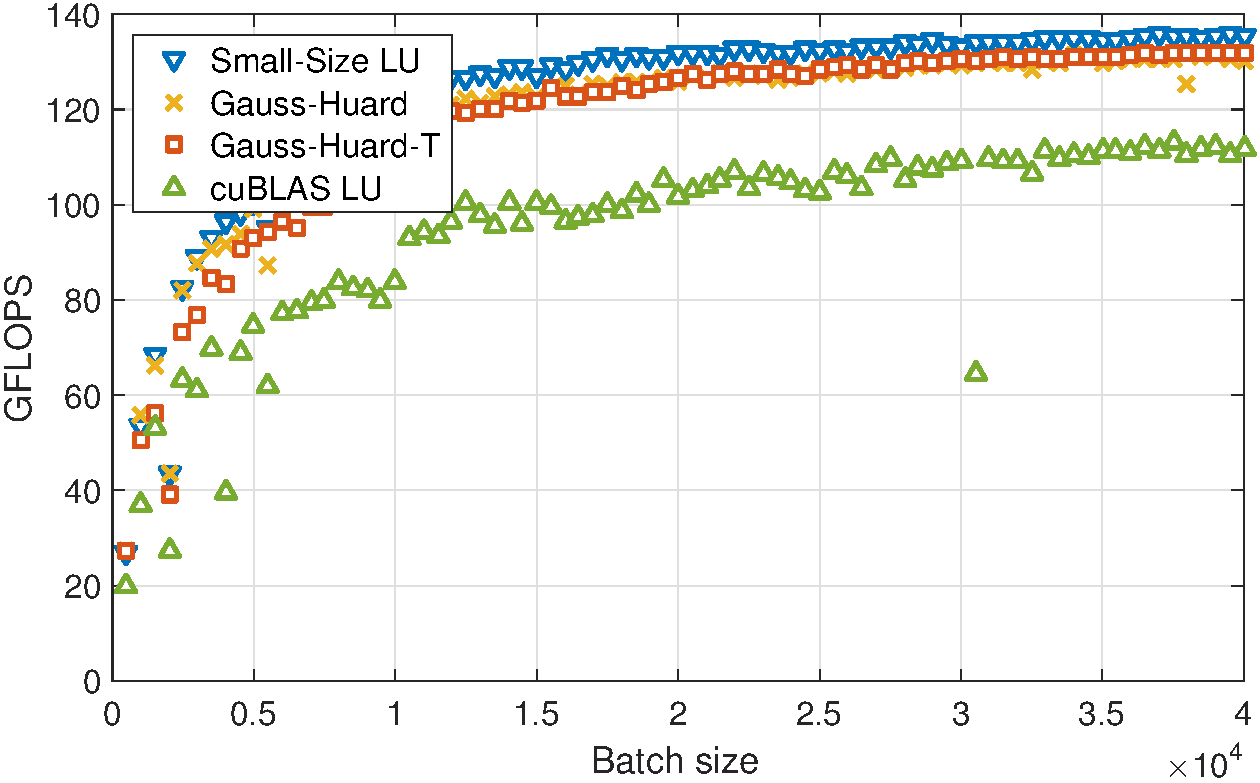
\includegraphics[width=.45\columnwidth]{plots/sgebjp_setup__lu_gje_gh_16.pdf}
&
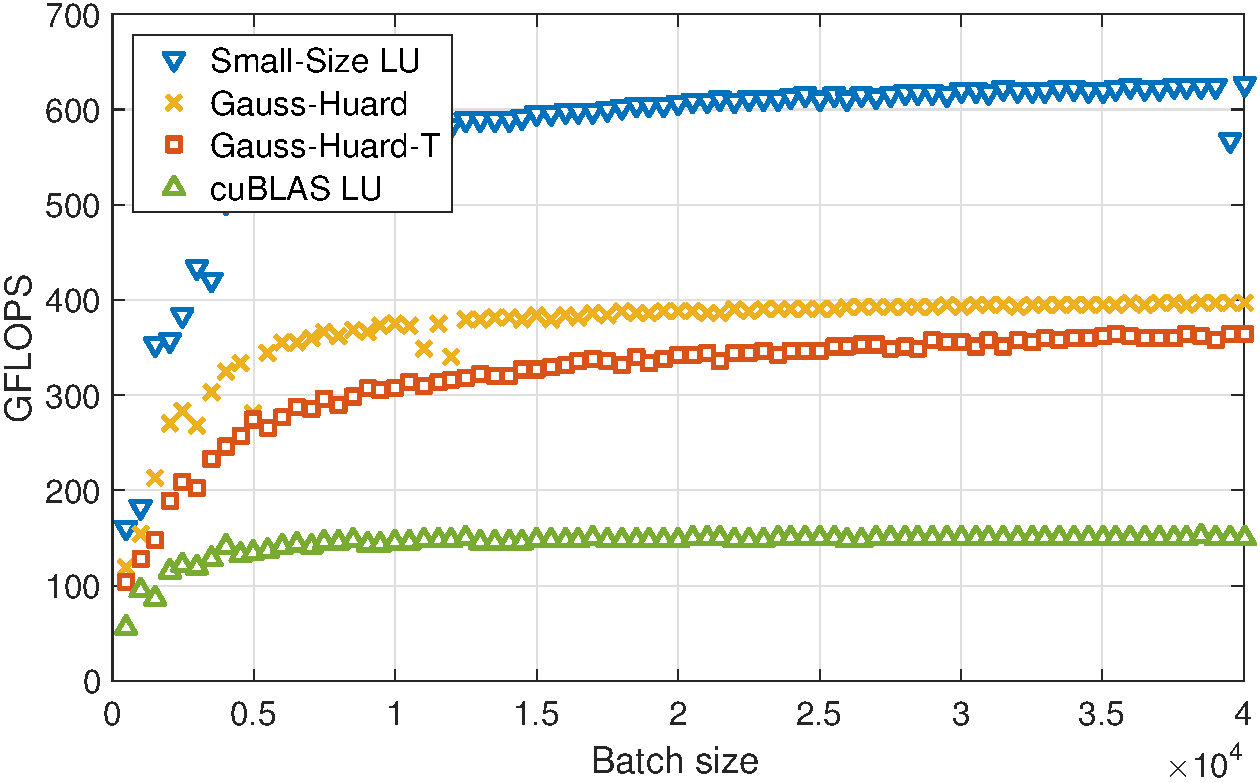
\includegraphics[width=.45\columnwidth]{plots/sgebjp_setup__lu_gje_gh_32.pdf}\\
\hline
Double-precision\\
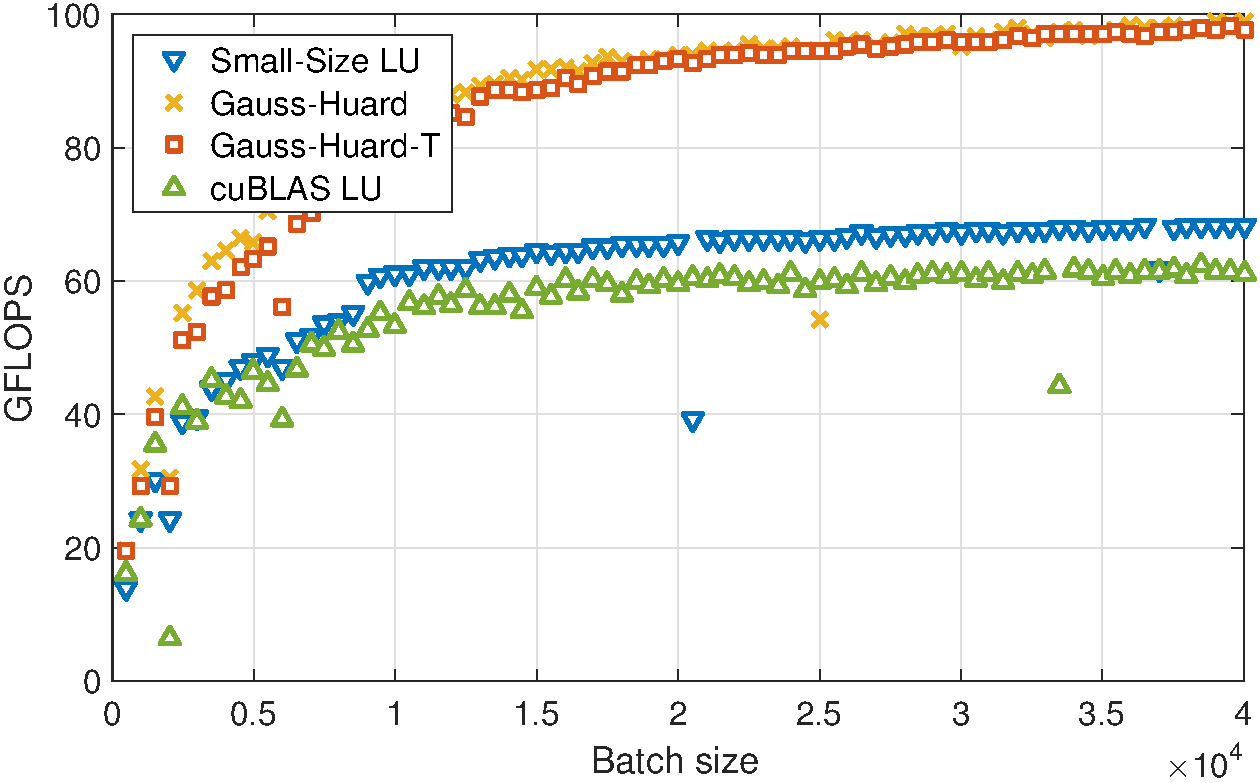
\includegraphics[width=.45\columnwidth]{plots/dgebjp_setup__lu_gje_gh_16.pdf}
&
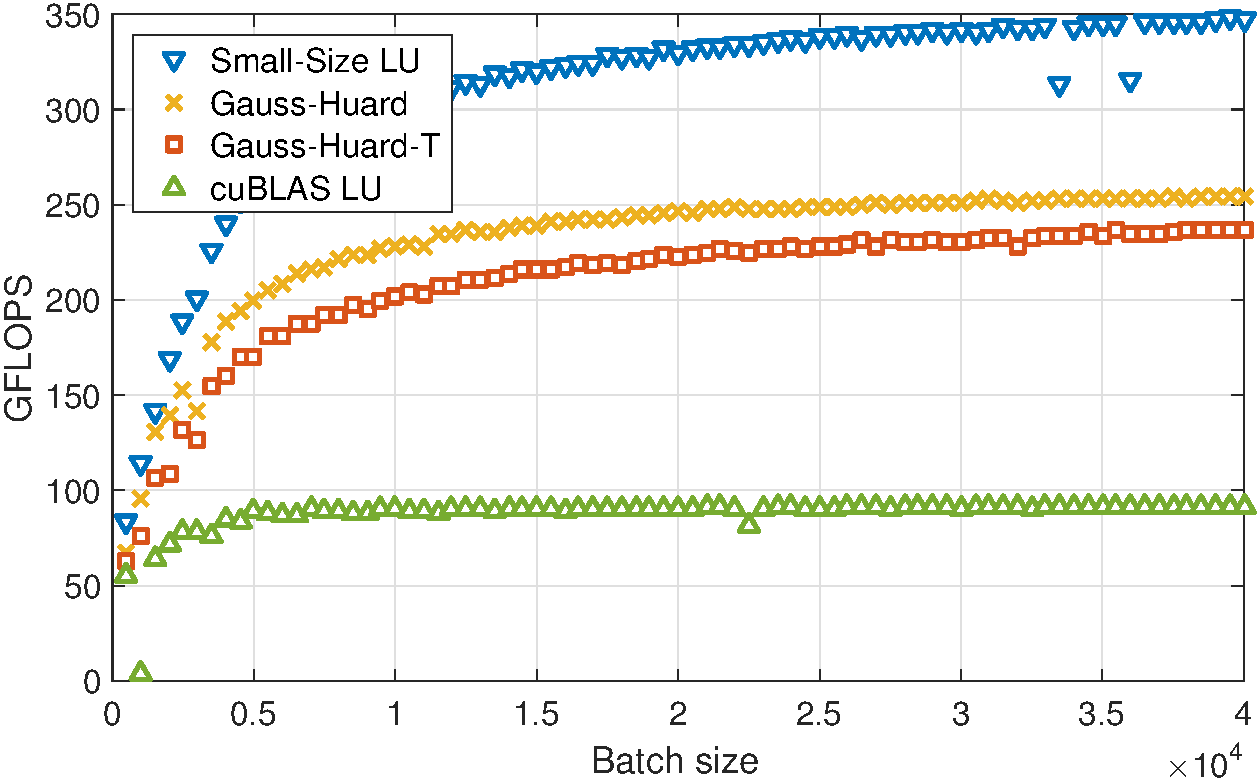
\includegraphics[width=.45\columnwidth]{plots/dgebjp_setup__lu_gje_gh_32.pdf}
\end{tabular}
\end{center}
\caption
[Performance of batched factorization routines depending on the batch size]
{%
Performance of batched factorization routines depending on the batch size.}
\label{2017-lu-block-jacobi:fig:performance}
\end{figure}


\section{Numerical Experiments}
\label{2017-lu-block-jacobi:sec:experiments}

\begin{figure}[t]
\begin{center}
\begin{tabular}{ll}
\hline
Single-precision & Double-precision\\
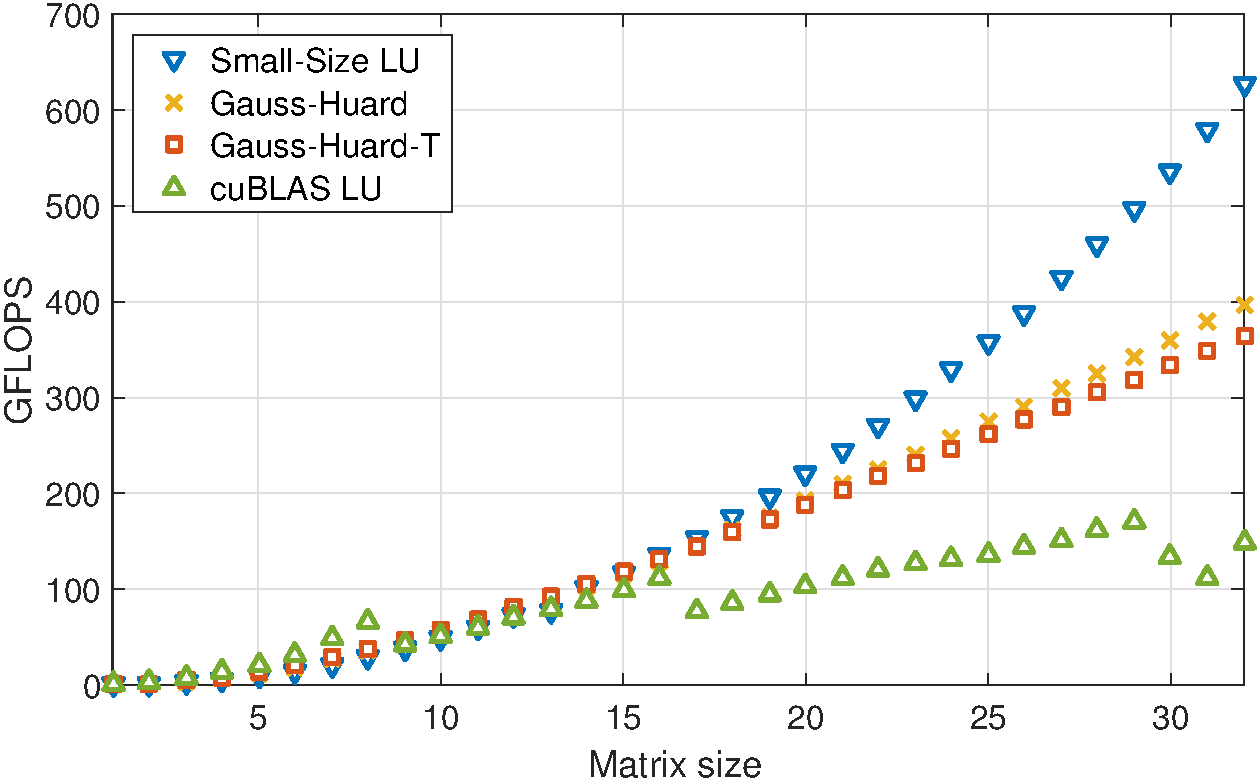
\includegraphics[width=.45\columnwidth]{plots/incsize_single.pdf}
&
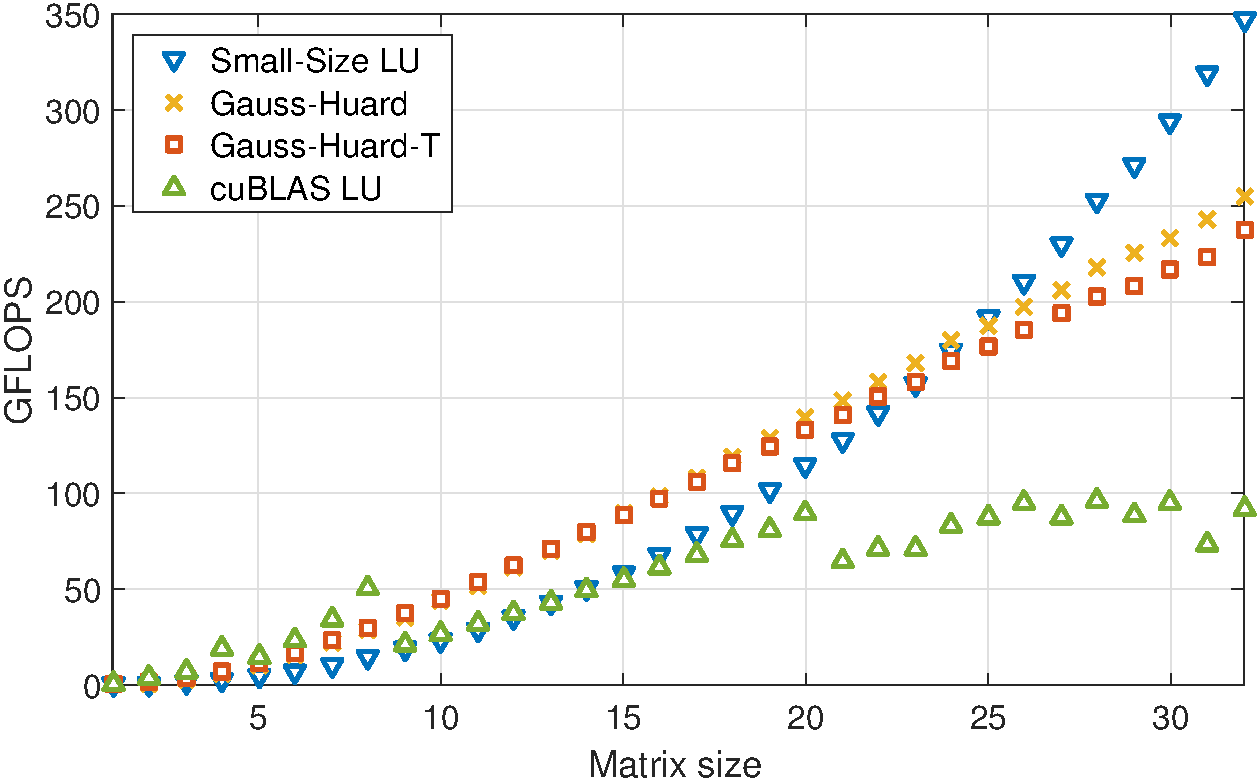
\includegraphics[width=.45\columnwidth]{plots/incsize_double.pdf}\\
\end{tabular}
\end{center}
\caption
[Performance of batched factorization routines depending on the size of the
matrices]
{%
Performance of batched factorization routines depending on the size of the matrices.
The batch size is fixed to 40,000 systems.
}
\label{2017-lu-block-jacobi:fig:performanceincsize}
\end{figure}

In this section we evaluate the performance of the batched LU factorization and triangular solve kernels tuned for small-size
problems
by comparing them
against alternative kernels offering similar functionality.
Concretely, our experimental analysis includes the following kernels:
\begin{itemize}
\item
\textit{Small-size LU:}
The batched LU factorization and triangular solve kernels developed as part of this work.
\item
\textit{Gauss-Huard:}
The batched factorization and triangular solve kernels based on GH~\cite{gh}.
\item
\textit{Gauss-Huard-T:}
The factorization in this routine is identical to the GH kernels, 
except in that the triangular systems are stored in a transpose access-friendly mode to
accelerate the triangular solves~\cite{gh}.
\item
\textit{cuBLAS LU:}
The batched LU factorization and triangular solve kernels available in NVIDIA's cuBLAS package (version 8.0).
\end{itemize}
We point out that the first three implementations
are part of the same software stack,
the kernel implementations are similar in design,
and received the same level of tuning.
cuBLAS is a vendor-implementation,
optimized specifically for the targeted architecture,
but its source is not available.
As variable block size is not supported by the batched kernels in cuBLAS,
the experiments involving them were conducted using
fixed block size for the entire batch.
This ensures a fair comparison and credible conclusions.

In addition to the evaluation of the LU factorization and triangular solve kernels, 
we assess the effectiveness of the computed preconditioner
integrated into the iterative IDR(4) solver for sparse linear systems~\cite{saad}.

\subsection{Hardware and software framework}
We employed an NVIDIA Tesla P100 GPU with full double-precision support in the experimentation
together with NVIDIA's GPU compilers that are shipped with the CUDA toolkit 8.0. 
Except for the {\sc getrf} and {\sc getrs}\footnote{Routine {\sc getrs} applies the sequence of permutations computed
by the LU factorization routine to the right-hand side vector, followed by two
triangular solves ({\sc trsv}).} 
routines taken from NVIDIA's cuBLAS library~\cite{cuda8.0}, 
all kernels
were designed to be integrated into the MAGMA-sparse library~\cite{magma}.
MAGMA-sparse was also leveraged to provide a testing environment, the block-pattern generation, and the sparse solvers.
Since the complete algorithm is executed on the GPU, the details of the CPU are
not relevant.

\subsection{Performance of batched factorization routines}

Figure~\ref{2017-lu-block-jacobi:fig:performance} compares the performance of the four
batched factorization routines in terms of GFLOPS (billions of flops per 
second).
The left-hand side plots in the figure report the performance
for a batch of matrices of size $16\times16$. 
The reference implementation for batched LU-based {\sc getrf} taken from NVIDIA's
cuBLAS library achieves about 110 GFLOPS in single-precision (top row).
In comparison, the small-size LU, Gauss-Huard and Gauss-Huard-T
all achieve about 130 GFLOPS for this case. In double-precision (bottom row), the performance
of the small-size LU is about 35\% lower than that of the GH-based
factorization routines, with the latter delivering about 100 GFLOPS. 
The scenario is different when the problem dimension is $32\times32$ (plots in the right-hand side of Figure~\ref{2017-lu-block-jacobi:fig:performance}):
The performance of Gauss-Huard-T is then about 5\% below that of Gauss-Huard,
and the small-size LU outperforms both routines by a significant margin, achieving up to
600 GFLOPS in single-precision and 350 GFLOPS in double-precision.
The cuBLAS counterpart providing the same functionality is 3.5$\times$ slower, delivering about 100 GFLOPS only.
The explanation for this block-size-dependent behavior
is an implementation detail, which will be corrected as part of future work.
Concretely, for block size $k < 32$, both the small-size LU and GH routines
operate with a matrix of size $32 \times 32$, padding the input with
zeros, but performing only the first $k$ steps of the factorization.
This benefits GH,
since it implements a ``lazy'' factorization,
while the ``eager'' (right-looking) algorithmic variant
selected for the LU factorization 
performs more flops than its GH counterpart for block-size $k<32$.
By optimizing the algorithms specifically for smaller block sizes,
we expect to observe the same behavior as that obtained for block size~32.

Figure~\ref{2017-lu-block-jacobi:fig:performanceincsize} reports the performance as a function of the problem size.
The results indicate that the non-coalescent writes in Gauss-Huard-T play a significant role only for 
problems of dimension larger than $16\times16$. For single-precision, 
this also corresponds  to the threshold from which
the small-size LU starts to outperform the GH-type factorizations. 
In double-precision, the small-size LU is slower than the GH-based factorizations
for problems smaller than $23\times23$.
The size-dependent results for cuBLAS LU reveal the system-specific optimizations:
local performance peaks can be identified for sizes 8, 16, and 
29 in single-precision arithmetic,
and for dimensions 8 and 20 in double-precision arithmetic. 
Although we do not tune for specific sizes by handling multiple problems per warp,
the small-size LU outperforms the cuBLAS LU for almost all sizes.


\begin{figure}[t]
\begin{center}
\begin{tabular}{ll}
Block size 16 & Block size 32\\
\hline
Single-precision\\
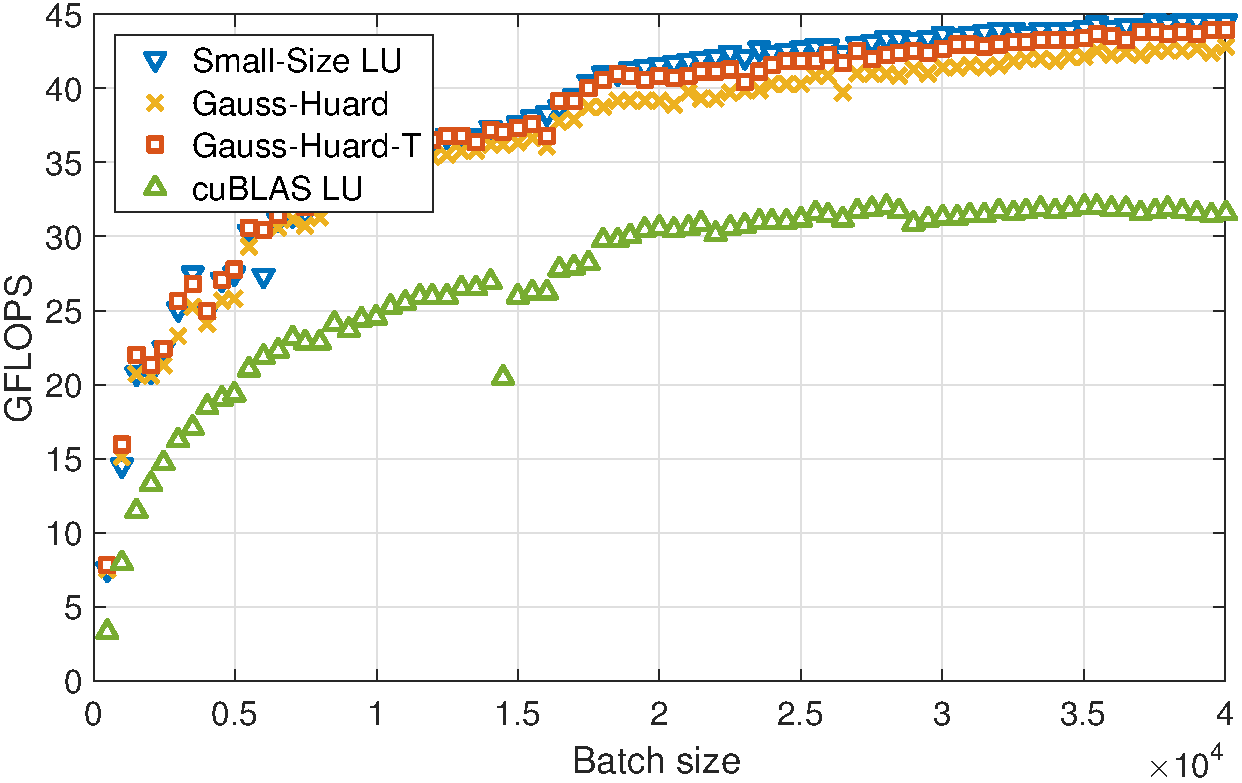
\includegraphics[width=.45\columnwidth]{plots/trsv_sgebjp_setup__lu_gje_gh_16.pdf}
&
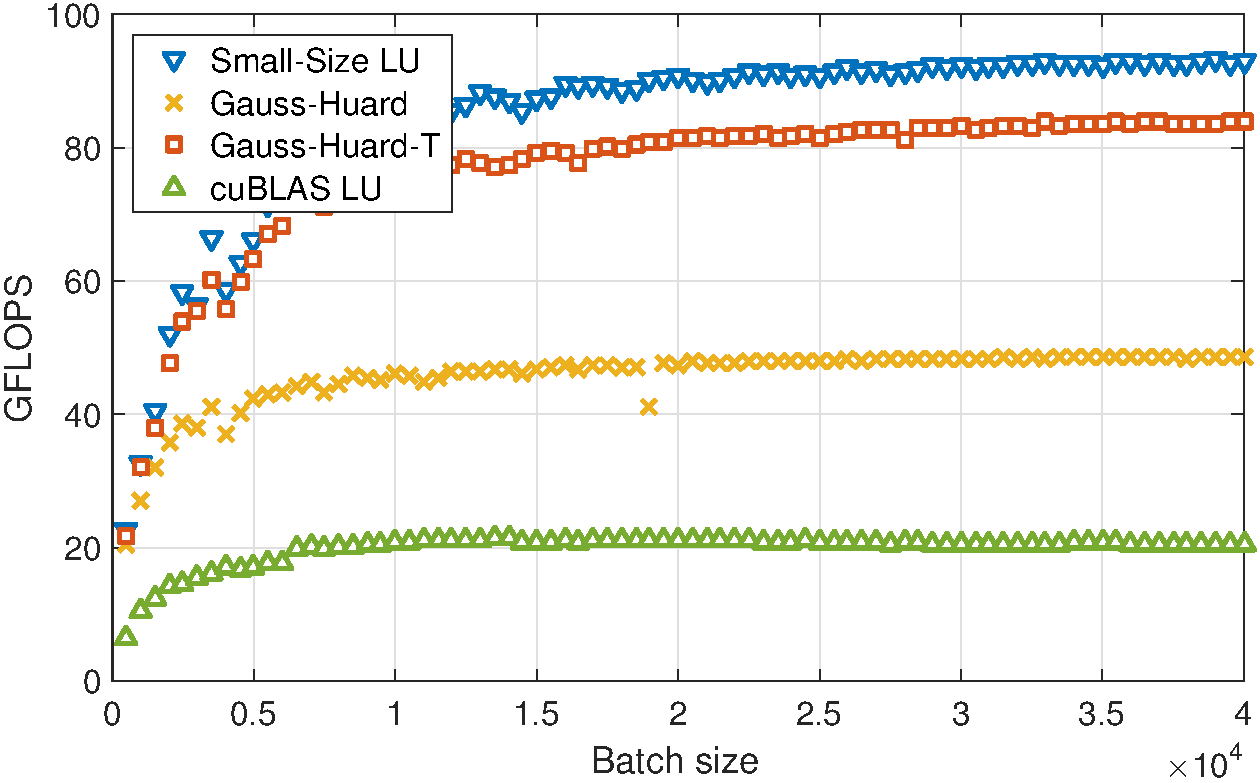
\includegraphics[width=.45\columnwidth]{plots/trsv_sgebjp_setup__lu_gje_gh_32.pdf}\\
\hline
Double-precision\\
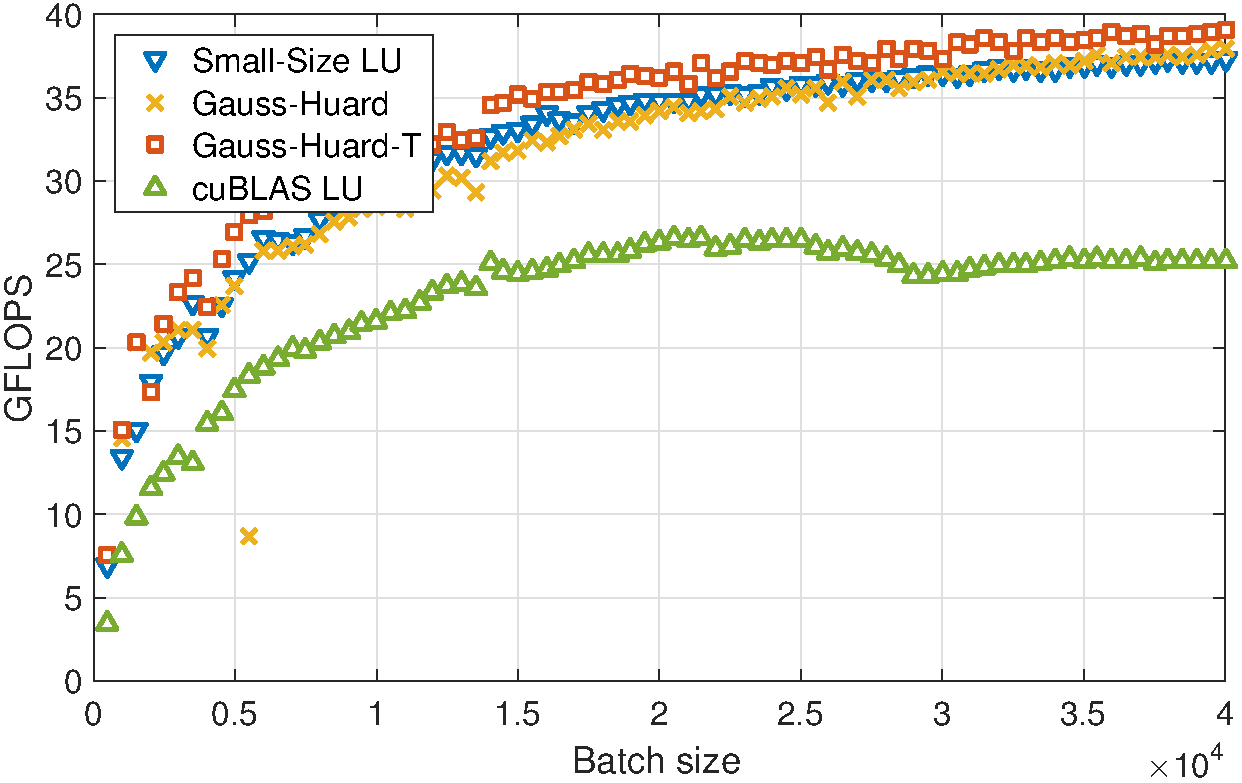
\includegraphics[width=.45\columnwidth]{plots/trsv_dgebjp_setup__lu_gje_gh_16.pdf}
&
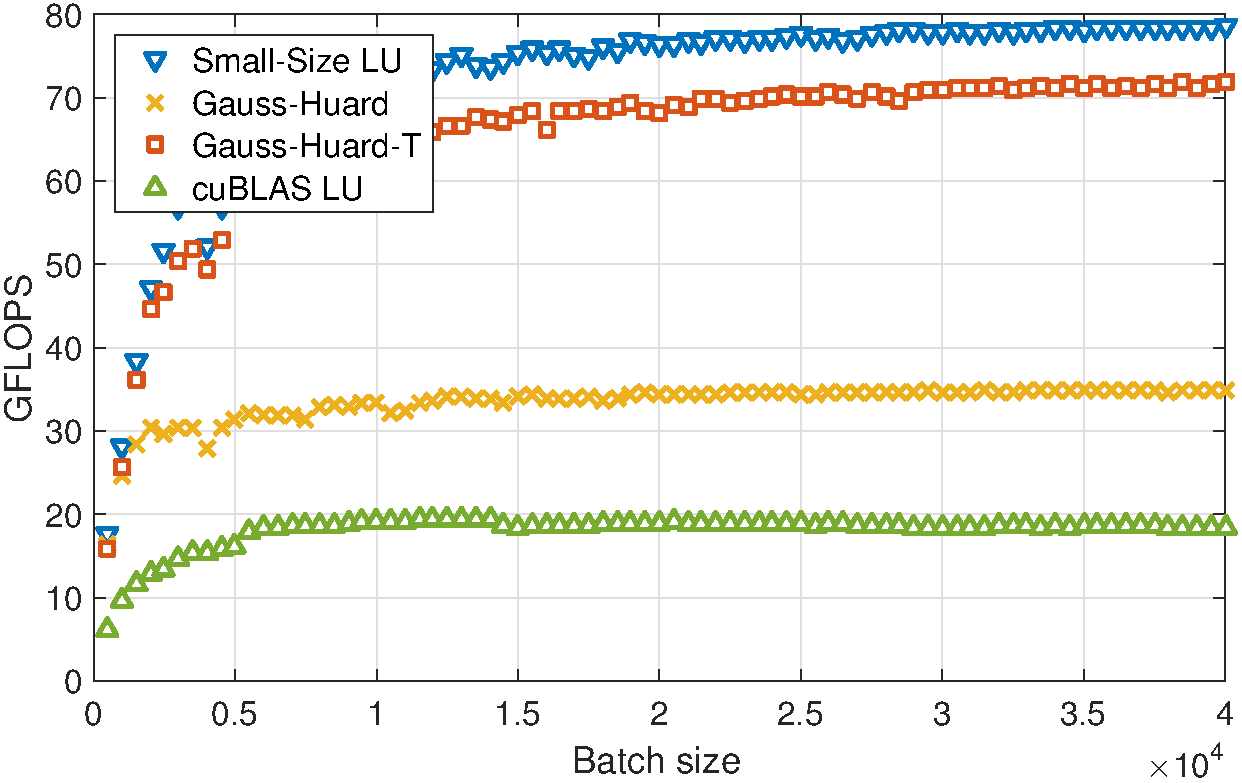
\includegraphics[width=.45\columnwidth]{plots/trsv_dgebjp_setup__lu_gje_gh_32.pdf}
\end{tabular}
\end{center}
\caption
[Performance of batched triangular solve routines depending on the batch size]
{%
Performance of batched triangular solve routines depending on the batch size.
}
\label{2017-lu-block-jacobi:fig:performancetrsv}
\end{figure}


\begin{figure}[t]
\begin{center}
\begin{tabular}{ll}
\hline
Single-precision & Double-precision\\
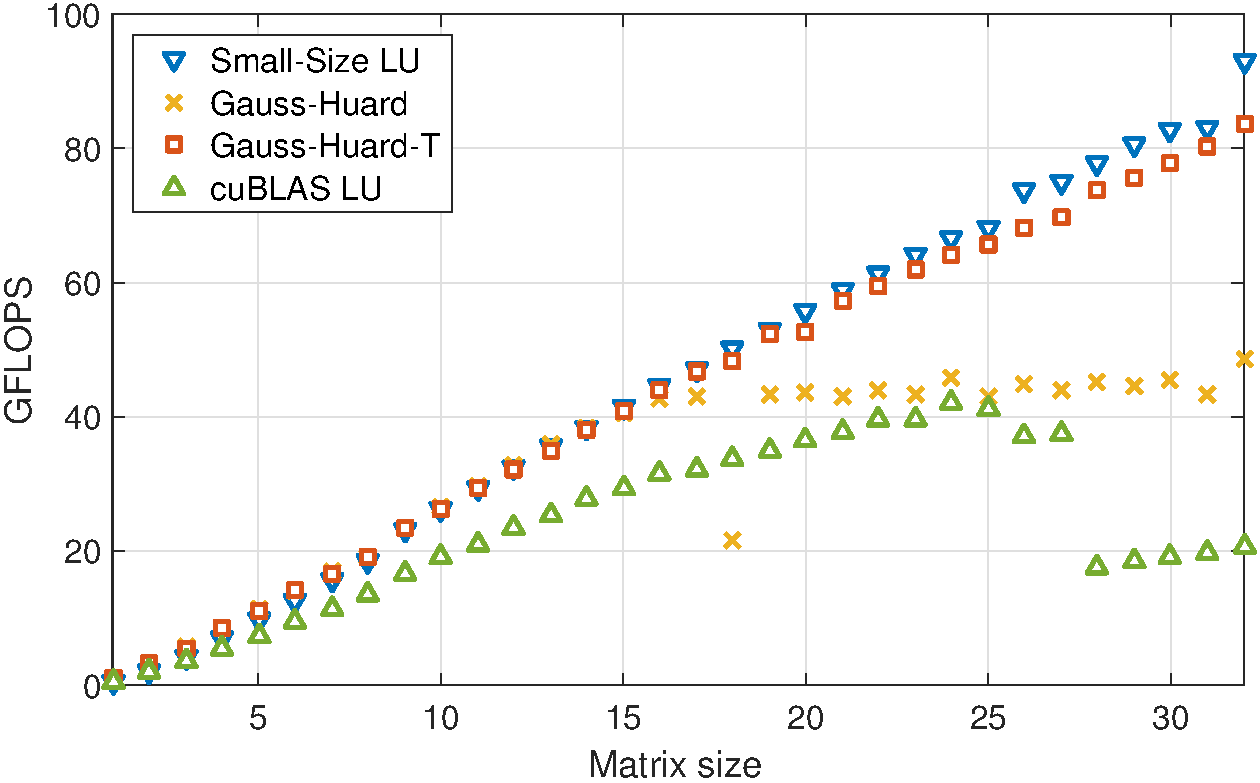
\includegraphics[width=.45\columnwidth]{plots/trsv_incsize_single.pdf}
&
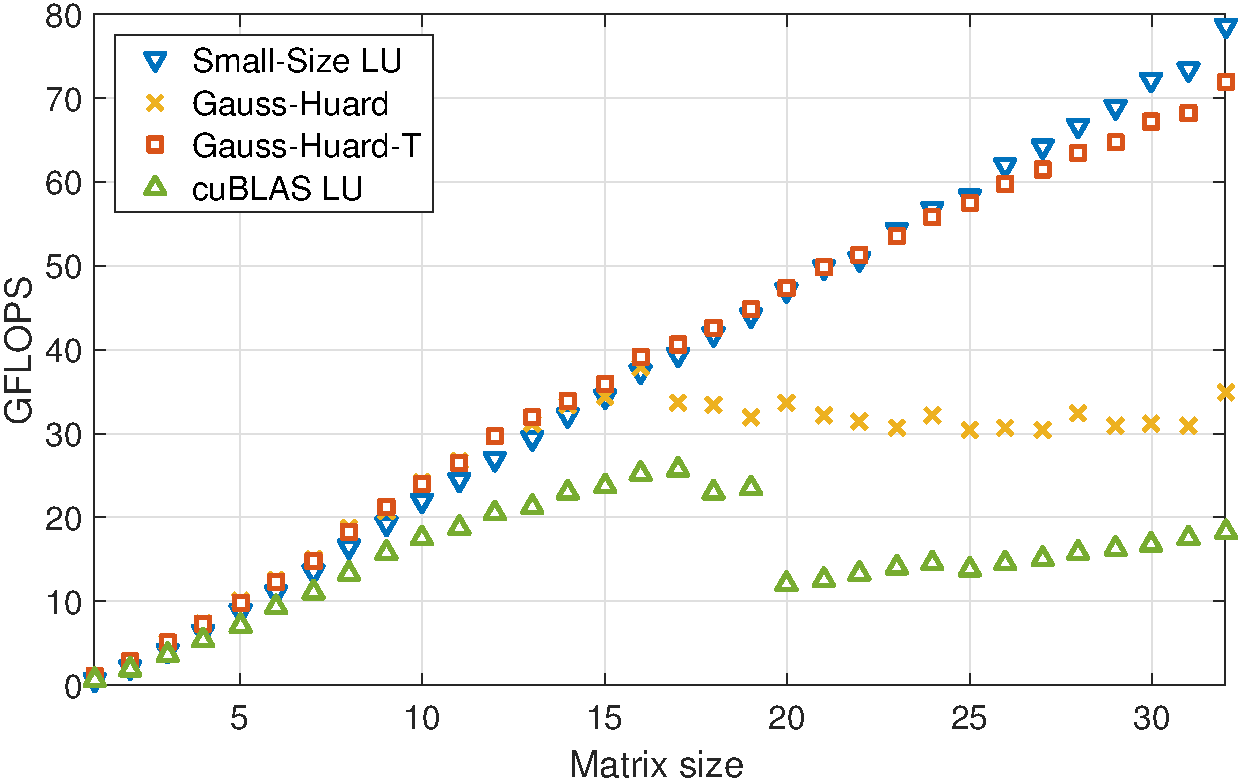
\includegraphics[width=.45\columnwidth]{plots/trsv_incsize_double.pdf}\\
\end{tabular}
\end{center}
\caption
[Performance of batched triangular solve routines depending on the size of the
matrices]
{%
Performance of batched triangular solve routines depending on the size of the matrices.
The batch size is fixed to 40,000 systems.
}
\label{2017-lu-block-jacobi:fig:performancetrsvincsize}
\end{figure}


\subsection{Performance of batched triangular solves}
We next employ the same notation in order to distinguish the different batched implementations of
the triangular solves that complement the factorization routines.
On the left-hand side plot in Figure~\ref{2017-lu-block-jacobi:fig:performancetrsv}, we assess the performance
of the triangular solves for a batch of matrices with size $16\times16$.
Unlike the factorization step, the performance for both GH variants and
the small-size LU are almost identical in single- as well as double-precision arithmetic
(44 GFLOPS and 37 GFLOPS, respectively).


For problems of size $32\times32$ (right-hand side plots in Figure~\ref{2017-lu-block-jacobi:fig:performancetrsv}), 
the more expensive Gauss-Huard-T factorization pays off
by accelerating the triangular solve from 47 GFLOPS (for Gauss-Huard) to 80+ GFLOPS
when using single-precision. In  double-precision the triangular solves of 
Gauss-Huard-T are also about twice faster (70 GFLOPS) than those associated with the
Gauss-Huard kernel (35 GFLOPS).
The small-size LU achieves 90+ GFLOPS in single-precision and close to 80 GFLOPS in double-precision.
This implies speed-up factors of 4.5$\times$ and 4$\times$ over cuBLAS, respectively.


Figure~\ref{2017-lu-block-jacobi:fig:performancetrsvincsize} analyzes the performance depending on the problem size.
Conversely to the factorization step, the non-coalescent reads in the Gauss-Huard triangular solves 
harm the performance for problems larger than $16\times16$.
For Gauss-Huard-T, the price of non-coalescent access was payed in the factorization step.
As a result, the Gauss-Huard-T triangular solves remain competitive with the
small-size LU triangular solves.
As in the factorization step, NVIDIA's {\sc getrs} seems to be optimized for problem of dimension smaller than 16;
nonetheless, this option achieves only a fraction of the performance of our small-size LU for all dimensions.



\begin{figure}[t]
\begin{center}
\begin{tabular}{c}
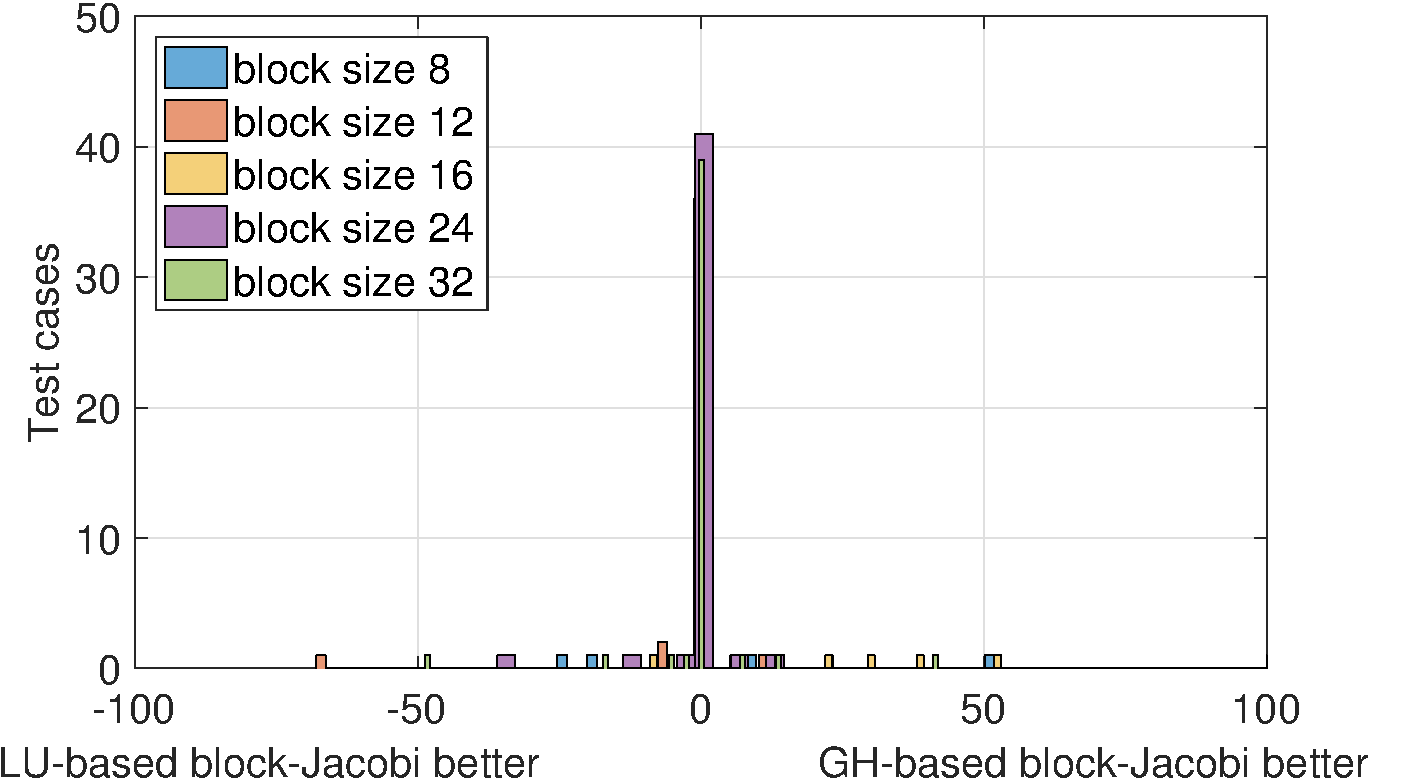
\includegraphics[width=.6\columnwidth]{plots/iteration_distribution_LU_GH_new}\\
\end{tabular}
\end{center}
\caption
[IDR(4) convergence using block-Jacobi preconditioning based on LU or GH]
{
IDR(4) convergence using block-Jacobi preconditioning based on LU factorization or GH-factorization: 
Iteration overhead in \% if LU provides the better preconditioner (left of center) or GH does (right of center).
}
\label{2017-lu-block-jacobi:fig:iterdist}
\end{figure}


\subsection{Analysis of block-Jacobi preconditioning for iterative solvers}

In this section we assess the efficiency of batched factorization routines in 
the context of block-Jacobi preconditioning.
For this purpose we enhance
an IDR(4) Krylov solver (taken from the MAGMA-sparse open source software package~\cite{ashes2016}) 
with a block-Jacobi preconditioner that is generated via 
batched factorization routines based on LU or GH, and applied in terms of triangular solves.
The diagonal block structure is generated via the supervariable blocking routines available in MAGMA-sparse, 
and we only vary the upper bound for the size of the diagonal blocks.
(At this point, we note that we do not include the cuBLAS batched LU 
in this comparison as it does not support variable problem size, which is needed for block-Jacobi preconditioning based on supervariable blocking.)
We perform our tests using a set of 48~selected matrices from the SuiteSparse matrix
collection~\cite{ufmc} (see the column labeled as ``Matrix in Table~\ref{2017-lu-block-jacobi:tab:idr4comparison}, and 
\url{http://www.cise.ufl.edu/research/sparse/matrices}). 
The test problems are listed along with some key characteristics in Table~\ref{2017-lu-block-jacobi:tab:idr4comparison},
and all carry some inherent block structure
which makes them attractive targets for block-Jacobi preconditioning.
We initialize the right-hand side vector with all its entries set to one,
start the iterative solver with an initial guess of zero,
and stop once the relative residual norm is decreased by six orders of magnitude.
We allow for up to 10,000 iterations. 

Although both the LU-based and GH-based factorizations present the same practical stability~\cite{Dek97}, 
we acknowledge the possibility of rounding effects. 
At this point, we note that rounding errors can have significant effect on
the convergence rate of the Krylov solver, and a more accurate factorization (preconditioner setup) does not inevitably result in
faster convergence of the preconditioned iterative solver. 
Figure~\ref{2017-lu-block-jacobi:fig:iterdist}
displays the convergence difference
of IDR(4) depending on 
whether the block-Jacobi preconditioner is based 
on LU or GH.
The x-axis of the histogram reflects the iteration overhead,
while the y-axis shows the number of test cases for which 
LU provided a ``better'' preconditioner (bars left of center) or
GH did (bars right of center).
For all block sizes, the majority of the problems is located in the center,
corresponding to those problem instances where both methods resulted in the same iteration count.
Furthermore, the histogram exposes a remarkable level of symmetry,
suggesting that, although rounding effects do occur, none of the
factorization strategies is generally superior.

In addition to the convergence rate (iteration count), we are also interested in comparing the 
practical performance of the two factorization strategies, in terms of execution time, in a block-Jacobi setting.
In Figure~\ref{2017-lu-block-jacobi:fig:runtime} we compare the total execution time (preconditioner setup time + iterative solver runtime)
of the IDR(4) solver 
using a block-Jacobi preconditioner based on either LU, GH or GH-T.
For this experiment, we use an upper bound of 32 for the supervariable agglomeration.
In most cases, the performance differences between the three options are negligible. 
Only due to rounding-error, and derived iteration count differences, one of the methods
becomes superior. The differences between GH and GH-T come from the faster
preconditioner generation
combined with a potentially-faster application of the latter.
The matrices are ordered in the x-axis according to the total execution time of the solver
and can be identified by the corresponding index in
Table~\ref{2017-lu-block-jacobi:tab:idr4comparison} (see column labelled as ``ID''). 
The 4 missing cases correspond to matrices for which the solver did not attain convergence.

To close this section, Table~\ref{2017-lu-block-jacobi:tab:idr4comparison} 
lists all test matrices along with the convergence behavior and execution time when
using different upper bounds for the Jacobi blocks in an IDR(4) solver preconditioned with the 
small-size LU-based block-Jacobi. The results suggest that larger block sizes typically improve the solver convergence
with respect to both iteration count and time-to-solution.




\begin{figure}[t]
\begin{center}
\begin{tabular}{c}
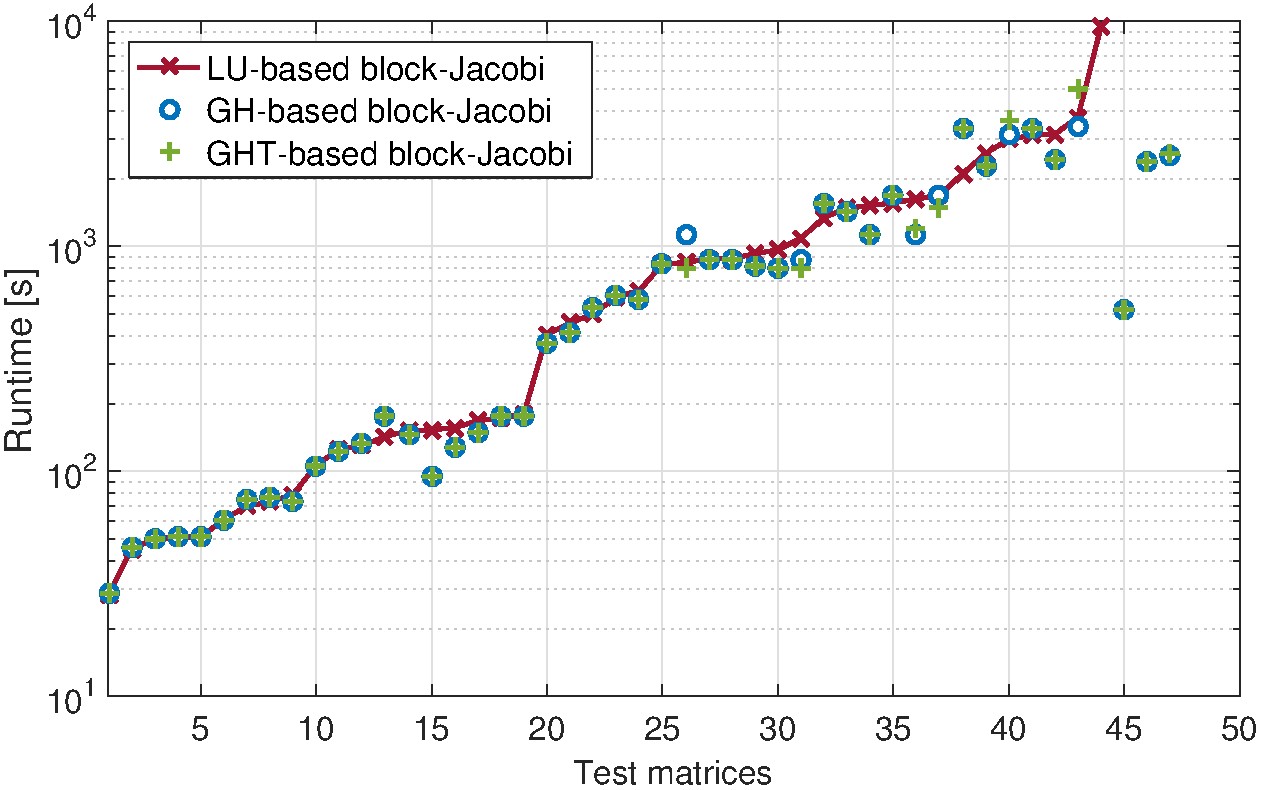
\includegraphics[width=.6\columnwidth]{plots/new_runtime_comparison_bs32}\\
\end{tabular}
\end{center}
\caption
[Execution time
for IDR(4) enhanced with block-Jacobi preconditioning based on LU or GH]
{
Total execution time (setup+solve) 
for IDR(4) enhanced with block-Jacobi preconditioning based on either LU or GH factorization.
The size of the distinct diagonal blocks is are adapted to the system matrix via supervariable 
blocking with 32 as upper bound. The matrix indices correspond to the values in the column 
labeled as ``ID'' in Table~\ref{2017-lu-block-jacobi:tab:idr4comparison}.
}
\label{2017-lu-block-jacobi:fig:runtime}
\end{figure}
